\graphicspath{{4integrals/asy/}}


\section{Integration}

At first glance, integration might appear straightforward; surely we can write the following?
\[
	\int_1^4 z^2\,\dz=\frac 13z^3\Big|_1^4 =\frac 13(4^3-1) =21
\]
In \emph{real} analysis such a statement reflects the equivalence of two distinct concepts:
\begin{itemize}\itemsep0pt
	\item[]\emph{Anti-derivatives}\quad $\frac 13z^3$ is an anti-derivative of $z^2$
	\item[]\emph{Definite Integrals}\quad The `area' under the curve $y=z^2$ on an interval $[0,z]$ equals $\frac 13z^3$
\end{itemize}
This amazing and important equivalence is suitably named the \emph{fundamental} theorem of calculus. But does it hold in \emph{complex} analysis? While anti-derivatives make immediate sense, definite integrals are more delicate. For instance, what should we mean by
\[
	\int_{3+i}^{4i} z^2\,\dz\text{ ?}
\]
A Riemann sum construction requires us to partition some \emph{curve} joining $3+i$ and $4i$; but which curve? Does it matter? These questions lead us to revisit \emph{contour/path integrals} from multi-variable calculus.

\subsection[Contour Integrals]{Functions of a Real Variable and Contour Integrals}\label{sec:contour}

We start by considering complex-valued functions of a \emph{real} variable $w:I\to\C$ where $I\subseteq\R$ is an interval; derivatives and definite integrals are built from those of their real and imaginary parts:
\[
	w'(t)=u'(t)+iv'(t),\qquad
	\int_a^bw(t)\,\dt=\int_a^bu(t)\,\dt+i\int_a^bv(t)\,\dt
	\tag{$a,b$ are \emph{real} or $\pm\infty$}
\]

\begin{examples}{}{basiccurvediff}
	\exstart If $w(t)=5t^2+it$, then
	\[
		w'(t)=10t+i,\qquad \int_1^2w(t)\,\dt=\int_1^25t^2\,\dt+i\int_1^2t\,\dt =\frac 73+\frac i2
	\]
	\begin{enumerate}\setcounter{enumi}{1}
		\item If $w(t)=t^2+e^{it}=t^2+\cos t+i\sin t$, then
		\[
			w'(t)=2t-\sin t+i\cos t,\qquad \int_0^{2\pi}w(t)\,\dt=\frac 13t^3+\sin t-i\cos t\Big|_0^{2\pi}=\frac 83\pi^3
		\]
		We see the natural extension of the (real) fundamental theorem here: $\frac 13t^3+\sin t-i\cos t$ is plainly an \emph{anti-derivative} of $w(t)$. This requires no proof since it applies separately to the real and imaginary parts of $w(t)$.
	\end{enumerate}
\end{examples}

Basic rules of integration are easily verified by separately considering real and imaginary parts.

\begin{lemm}{}{basiccalcrealvar}
	$\bullet$ \ Linearity: \ if $k\in\C$, then $\diff tkw(t)=kw'(t)$ and $\int_a^bkw(t)\,\dt=k\int_a^bw(t)\,\dt$
	\begin{itemize}
	  \item Product rule: \ $\diff tw(t)z(t)=w'(t)z(t)+w(t)z'(t)$
	  \item Chain rule: \ If $s(t)$ is a \emph{real} function then $\diff tw\bigl(s(t)\bigr)=w'\bigl(s(t)\bigr)s'(t)$
	\end{itemize}
\end{lemm}

\goodbreak


\emph{Complex} substitutions are more subtle, so we provide a proof.

\begin{lemm}{Complex Chain Rule}{chainsubs}
	Suppose $w(t)=F\bigl(z(t)\bigr)$ where
	\begin{itemize}
	  \item $z(t)=x(t)+iy(t)$ is differentiable at $t$, and,
	  \item $F(z)=u(x,y)+iv(x,y)$ is holomorphic at $z(t)$
	\end{itemize}
	Then $w$ is differentiable at $t$, and $w'(t)=F'\bigl(z(t)\bigr)z'(t)$.\smallbreak
	If $z'(t)$ is integrable on $[a,b]$ and $F$ holomorphic on $z([a,b])$, we can put this in integral form
	\[
		\int_a^bF'\bigl(z(t)\bigr)z'(t)\,\dt %=\int_a^b\diff tF\bigl(z(t)\bigr)\,\dt
		=F\bigl(z(b)\bigr)-F\bigl(z(a)\bigr)
	\]
\end{lemm}



\begin{proof}
	Apply the multi-variable chain rule from real calculus and the Cauchy--Riemann equations:
	\begin{align*}
		\diff[w]{t}&=\diff[u]{t}+i\diff[v]{t} = \partials[u]{x}\diff[x]{t}+\partials[u]{y}\diff[y]t
			+i\left(\partials[v]{x}\diff[x]{t}+\partials[v]{y}\diff[y]{t}\right) \\
			&=(u_x+iv_x)\diff[x]{t}+i(v_y-iu_y)\diff[y]{t} 
		= (u_x+iv_x)\left(\diff[x]{t}+i\diff[y]{t}\right) \tag{Cauchy--Riemann}\\
		&= F'\bigl(z(t)\bigr)z'(t) \tag*{\qedhere}
	\end{align*}
\end{proof}

\begin{examples}{}{}
	\exstart Let $w(t)=e^{t-it^2}=F\bigl(z(t)\bigr)$ where $F(z)=e^z$ and $z(t)=t-it^2$. Then
	\[
		w'(t) =e^{t-it^2}\diff t(t-it^2) =e^{t-it^2}(1-2it)
	\]
	Compare with the method of Example \ref{ex:basiccurvediff} which gives the same result, if more slowly
	\[
		w'(t) =\diff t(e^t\cos t^2-ie^t\sin t^2) =e^t(\cos t^2-2t\sin t^2)-ie^t(\sin t^2+2t\cos t^2)
	\]
	\begin{enumerate}\setcounter{enumi}{1}
		\item Since $w(t)=F\bigl(z(t)\bigr) =\frac 1{10}(1-t^2+it)^{10}$ has $w'(t)=(i-2t)(1-t^2+it)^9$, we see that
		\[
			\int_0^1(i-2t)(1-t^2+it)^9\,\dt =\frac 1{10}(1-t^2+it)^{10}\bigg|_0^1 =\frac{i^{10}-1}{10} =-\frac 15
		\]
		This would be horrific if we instead had to multiply out to find the real and imaginary parts!
		\item Sometimes the real and imaginary part approach is simply not tenable,
		\[
			\int_0^1 3it\sqrt{1+it^2}\,\dt =(1+it^2)^{3/2}\Big|_0^1 =(1+i)^{3/2}-1 =2\sqrt 2\polar{3\pi i}8-1
		\]
		We evaluate using the principal square root since $1+it^2$ lies in the first quadrant.
	\end{enumerate}
\end{examples}
\goodbreak

While most of the basic rules of real calculus translate to complex-valued functions of a real variable, not everything goes through. Be particularly careful of existence results such as the mean value theorem which apply perfectly well to real and imaginary parts, but not to the whole\ldots
\goodbreak


\boldsubsubsection{Contours and Contour Integrals}

We want to integrate complex functions along curves. But what sort of curves?

\begin{defn}{}{}
	A \emph{smooth arc} is an oriented curve $C$ in the complex plane for which there exists a \emph{regular parametrization}; a differentiable function $z:[a,b]\to\C$ such that:\vspace{-2pt}
	\begin{enumerate}\itemsep2pt
	  \item $z([a,b])=C$ where $z(a)$ is the \emph{start} of the curve and $z(b)$ is the \emph{end}.
	  \item $z'(t)$ is \emph{continuous}\footnotemark{} on $[a,b]$ and \emph{non-zero} on $(a,b)$.
	\end{enumerate}
	A \emph{contour} is a piecewise smooth arc $C$ consisting of finitely many smooth arcs joined end-to-end. A parametrization $z(t)$ of $C$ is therefore continuous with piecewise continuous derivative.\smallbreak
	If we \emph{reverse the orientation} of a contour $C$, the resulting contour is labelled $-C$.\smallbreak
	Additionally, we say that a contour is:\vspace{-2pt}
	\begin{itemize}\itemsep2pt
	  \item \emph{Closed} if it starts and ends at the same point, $z(a)=z(b)$;
	  \item \emph{Simple} if it does not cross itself ($z$ is injective, $z(t)=z(s)\implies t=s$).
	  \item \emph{Positively oriented} if it is simple, closed and traversed counter-clockwise.
	\end{itemize}
\end{defn}

\footnotetext{%
	Since $\nm{z'(t)}$ is bounded on $[a,b]$, the arc-length $\int_a^b\nm{z'(t)}\,\dt$ is finite. This extends to any contour.
}

\begin{examples}{}{contourintro}
	Here are three contours with explicit parametrizations:\vspace{-5pt}
	\begin{center}
		\begin{tabular}{c@{\qquad}c@{\qquad}c}
			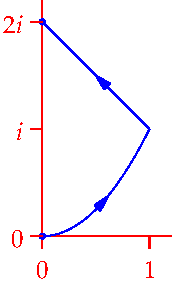
\includegraphics[scale=0.9]{contours-ex1}
			&
			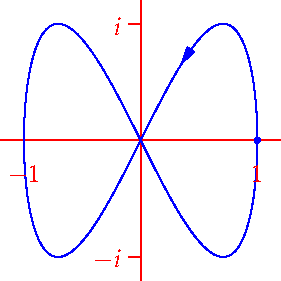
\includegraphics[scale=0.9]{contours-ex2}
			&
			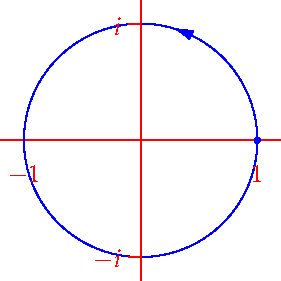
\includegraphics[scale=0.9]{contours-ex3}
			\\
			Simple, piecewise
			&
			Closed, non-simple
			&
			Positively oriented
			\\[2pt]
			$z=\begin{cases}
			t+it^2&t\in[0,1]\\
			2-t+it&t\in[1,2]
			\end{cases}$
			&
			$z=\cos t+i\sin 2t$, $t\in[0,2\pi]$
			&
			$z=e^{it}$, $t\in[0,2\pi]$
		\end{tabular}
	\end{center}
\end{examples}

\begin{defn}{}{}
	Let $C$ be a contour parametrized by $z:[a,b]\to\C$ and suppose that $f(z)$ is a complex function defined on the range of $z$. The \emph{contour integral} of $f(z)$ along $C$ is
	\[
		\int_Cf=\int_Cf(z)\,\dz:=\int_a^bf\bigl(z(t)\bigr) z'(t)\,\dt
	\]
	This is often written $\oint_Cf$ if $C$ is positively oriented (simple and closed).
\end{defn}

We plainly require, and assume from now on by default, that the function $f\bigl(z(t)\bigr)z'(t)$ is integrable on the \emph{real interval} $[a,b]$; indeed we typically assume that this expression is \emph{piecewise continuous}. %As we'll see shortly, the choice of parametrization $z(t)$ of $C$ is irrelevant.
\goodbreak



\begin{examples}{}{basiccontour}
	We evaluate several contour integrals.
	\begin{enumerate}
	  \begin{minipage}[t]{0.65\linewidth}\vspace{-5pt}
		  \item For the contour $\textcolor{Green}{C_1}$ parametrized by $z(t)=t+it^2$, $t\in[0,1]$, we compute
		  \begin{align*}
			  \int_{\textcolor{Green}{C_1}}z\,\dz&=\int_0^1z(t)z'(t)\,\dt=\int_0^1(t+it^2)(1+2it)\,\dt\\
			  &=\int_0^1t-2t^3+3it^2\,\dt=i
		  \end{align*}
		  
		  \item For the contour $\textcolor{blue}{C_2}$ with $z(t)=e^{it}$ with $t\in[0,\pi]$,
		  \[
		  	\int_{\textcolor{blue}{C_2}}\frac 1z\,\dz =\int_0^{\pi}\frac{ie^{it}}{e^{it}}\,\dt =\pi i
		  \]
	  \end{minipage}
	  \hfill
	  \begin{minipage}[t]{0.34\linewidth}\vspace{-10pt}
	  	\flushright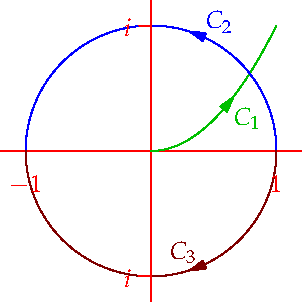
\includegraphics{contours-ex4}
	  \end{minipage}\par
	  \vspace{-10pt}
	  
	  \item[]
	  \[
	  	\int_{\textcolor{blue}{C_2}}z^2+1\,\dz =\int_0^{\pi}(e^{2it}+1)ie^{it}\,\dt =\frac i{3i}e^{3it}+\frac i{i}e^{it}\Big|_0^{\pi}= \frac 13(e^{3\pi i}-1)+e^{\pi i}-1=-\frac 83
	  \]
	  \item We compute the same integrals as the previous example, but over the lower semi-circle $\textcolor{Brown}{C_3}$ parametrized by $z(t)=e^{-it}$ with $t\in[0,\pi]$. This time
	  \begin{gather*}
	  	\int_{\textcolor{Brown}{C_3}}\frac 1z\,\dz =\int_0^{\pi}\frac{-ie^{-it}}{e^{-it}}\,\dt =-\pi i\\
	  	\int_{\textcolor{Brown}{C_3}}z^2+1\,\dz =\int_0^{\pi}(e^{-2it}+1)(-ie^{-it})\,\dt =\frac{-i}{-3i}e^{-3it}+\frac{-i}{-i}e^{-it}\Big|_0^{\pi}=-\frac 83
	  \end{gather*}
	  The \emph{sign} of one integral changed but the other did not! We'll return to this problem shortly\ldots
	\end{enumerate}
\end{examples}


Before considering more examples we develop some of the basic properties of contour integrals. Several are immediate from our earlier discussion, for instance linearity:
\[
	\int_C\bigl(af(z)+bg(z)\bigr)\,\dz=a\int_Cf(z)\,\dz+b\int_Cg(z)\,\dz
\]
Of more importance are the following:

\begin{thm}{Basic rules for contour integrals}{basiccontour}
	Suppose $C$ is a contour parametrized by $z(t)$.\par
	\begin{minipage}[t]{0.75\linewidth}\vspace{-5pt}
		\begin{enumerate}
		  \item If $C=C_1\cup C_2$, where $\textcolor{blue}{C_1}$ and $\textcolor{orange}{C_2}$ are contours such that the end of the first is the start of the second, then
		  \[
		  	\int_Cf(z)\,\dz=\int_{C_1}f(z)\,\dz+\int_{C_2}f(z)\,\dz
		  \]
		  \item $\int_Cf$ is independent of (orientation-preserving) parametrization.
		  \item Reversing orientation changes the sign of the integral: $\int_{-C}f=-\int_Cf$.
		\end{enumerate}
	\end{minipage}
	\hfill
	\begin{minipage}[t]{0.24\linewidth}\vspace{-5pt}
		\flushright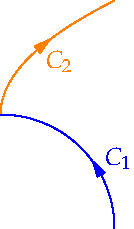
\includegraphics{contours-ex5}
	\end{minipage}
\end{thm}


\begin{example}{}{int2pii}
	By the previous example and part 3 of the Theorem, if $C$ is the unit circle centered at the origin, then $\oint_C\frac 1z\,\dz=2\pi i$. This can also be verified  directly.
\end{example}
\goodbreak



\begin{proof}
	Part 1 follows from the well-known property $\int_a^b=\int_a^c+\int_c^b$ of real integrals. Armed with this, it is enough to check the other parts for a single smooth arc $C$.\vspace{-5pt}
	\begin{enumerate}\setcounter{enumi}{1}
	  \item Suppose $z:[a,b]\to\C$ and $w:[\alpha,\beta]\to \C$ are parametrizations of $C$. Then $w\bigl(s(t)\bigr)=z(t)$ for some continuously differentiable $s$ with \emph{positive} derivative. Now compute,
		\begin{gather*}
			z'(t)=w\bigl(s(t)\bigr)s'(t),\qquad s(a)=\alpha,\quad s(b)=\beta,\quad\text{from which,}\\
			\begin{aligned}
				\int_a^bf\bigl(z(t)\bigr)z'(t)\,\dt &=\int_a^bf\bigl(w(s(t))\bigr)w'(s(t))\diff[s]{t}\,\dt =\int_{s(a)}^{s(b)} f\bigl(w(s)\bigr)w'(s)\,\ds\\
				&=\int_{\alpha}^{\beta} f\bigl(w(s)\bigr)w'(s)\,\ds
			\end{aligned}
		\end{gather*}\vspace{-20pt}
		\item This is almost identical, except that $-C$ requires a reparametrization $w(s)$ with $s'<0$, $s(a)=\beta$ and $s(b)=\alpha$. The upshot is that the limits flip on the final integral:
		\[
			\int_Cf=\int_a^bf\bigl(z(t)\bigr)z'(t)\,\dt =\int_{\beta}^{\alpha} f\bigl(w(s)\bigr)w'(s)\,\ds =-\int_{\alpha}^{\beta} f\bigl(w(s)\bigr)w'(s)\,\ds =-\int_{-C}f \tag*{\qedhere}
		\]
	\end{enumerate}
\end{proof}


% \footnote{If $w=u+iv$ is continuous on $[a,b]$ and differentiable on $(a,b)$, then $\exists \xi,\eta\in(a,b)$ such that
% \[\frac{w(b)-w(b)}{b-a}= \frac{u(b)-u(a)}{b-a} +i\frac{v(b)-v(a)}{b-a}=u'(\xi)+iv'(\eta)\]
% There is no reason for $\xi$ to equal $\eta$, so we should not expect the right hand side to equal $w'(\xi)$.}


\boldinline{Contour Integrals of multi-valued functions}

If a function is multi-valued, we must specify a \emph{branch} before integrating. It is acceptable to have the contour start and/or finish on the branch cut.\footnote{We extend the integrand continuously: recall that if $g(t)$ is \emph{uniformly continuous} on a bounded open interval $(a,b)$, then it has a continuous extension to the closed interval $[a,b]$ and we can therefore define $\int_a^bg(t)\,\dt$.}

\begin{examples}{}{sqrootint}
	\exstart Compute $\oint_{C_1}z^{1/2}\,\dz$ over the unit circle using the principal square root.
	\begin{enumerate}\setcounter{enumi}{1}
		\begin{minipage}[t]{0.65\linewidth}\vspace{-7pt}
			\item[]Since the question specifies the principal branch, we must must start and finish the contour at $z=-1$. Parametrize via $z(t)=e^{it}$ where $t\in(-\pi,\pi)$. Since
			\[
				\sqrt{z(t)}\,z'(t)=\polar{it}2ie^{it}=i\polar{3it}2
			\]
			is continuous on $[-\pi,\pi]$, we compute
			\[
				\int_{C_1}z^{1/2}\,\dz=\int_{-\pi}^\pi i\polar{3it}2\,\dt =\frac 23\polar{3it}2\Big|_{-\pi}^{\pi} =\frac 23(\polar{3\pi i}2-\polarn{3\pi i}2)=-\frac{4i}3
			\]
		
			\item Find $\int_{C_2}z^i\,\dz$ over the unit semi-circle shown using $\operatorname{P.V.}z^i$.\smallbreak
			Let $z(t)=e^{it}$ where $t\in[0,\pi]$. Since
			\[
				z^iz'=e^{i\Log z}z'=\exp\left(i(it)\right)ie^{it}=ie^{(i-1)t}
			\]
			is continuous when $0\le t\le \pi$, we have
		\end{minipage}
		\hfill
		\begin{minipage}[t]{0.34\linewidth}\vspace{-10pt}
			\flushright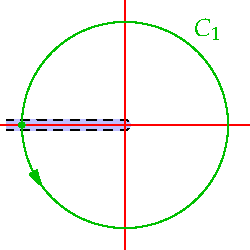
\includegraphics{contour-branch2}\bigbreak\medbreak
			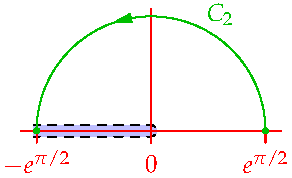
\includegraphics{contour-branch3}
		\end{minipage}
		\[
			\int_{C_2}z^i\,\dz=\int_0^\pi ie^{(i-1)t}\,\dt =\frac{i}{i-1}\bigl(e^{(i-1)\pi}-1\bigr) =\frac{i-1}{2}\bigl(1+e^{-\pi}\bigr)
		\]
	\end{enumerate}
\end{examples}


\textcolor{red}{Warning!} Things are more difficult if we allow a contour to \emph{cross} a branch cut, since we'd then have to work with multiple branches simultaneously. We won't do this.
\goodbreak


\begin{exercises}
	\exstart Evaluate the derivatives and integrals:
	\begin{enumerate}\setcounter{enumi}{1}
	  \item[]\begin{tabular}[t]{r@{\ \ }l@{\qquad}r@{\ \ }l@{\qquad}r@{\ \ }l}
		  (a)&
		  $\displaystyle\diff t\left[\sin t+i\sqrt t\right]$&
		  (b)&
		  $\displaystyle\diff t(i+t^3)^2$&
		  (c)&
		  $\displaystyle\int_0^1e^{\pi it}\,\dt$\\[10pt]
			(d)&
			$\displaystyle\int_0^{\pi/2} e^{it}(1+e^{it})^2\,\dt$&
		  (e)&
		  $\displaystyle\int_0^1(i-t)^6\,\dt$&
			(f)&
			$\displaystyle\int_0^{\pi} (i-1)\cos\bigl((1+i)t\bigr)\,\dt$
	  \end{tabular}
	  
	  
	  \item Show that if $m,n\in\Z$, then
	  \[
	  	\int_0^{2\pi}e^{imt}e^{-int}\,\dt=2\pi\delta_{mn}
	  \]
	  where $\delta_{mn}=1$ when $m=n$ and 0 otherwise. Do this two ways:
	  \begin{enumerate}
	    \item Using the exponential law and the chain rule/substitution.
	    \item By multiplying out and working with real and imaginary parts.
	  \end{enumerate}
	  
	  
	  \item Use the chain rule to evaluate the integral $\int_0^xe^{(1+i)t}\,\dt$.\\
	  Hence find both $\int_0^xe^t\cos t\,\dt$ and $\int_0^xe^t\sin t\,\dt$ \emph{without} using integration by parts.
	  
	  
	  \item Prove the product rule for functions of a real variable:
	  \[
	  	\diff t(wz)=w'z+wz'
	  \]
	 	(\emph{Hint: let $w(t)=u(t)+iv(t)$, \ $z(t)=x(t)+iy(t)$ and multiply out\ldots})
	  
	  
	  \item Check that the mean value theorem fails for the function $w(t)=\sqrt t+it^2$ on the interval $[0,1]$. That is, there is no $\xi\in(0,1)$ for which $w'(\xi)=\frac{w(1)-w(0)}{1-0}$.
	  
	  
	  \item Justify the integral form of the complex chain rule by considering the real and imaginary parts of $F$. What facts from real calculus are you using?
	  
	  
	  \item Evaluate each contour integral $\int_Cf(z)\,\dz$ by explicitly parametrizing $C$:
		\begin{enumerate}
	    \item $f(z)=z^2$;\quad $C$ is the straight line from $z=1$ to $z=i$.
	    \item $f(z)=z$;\quad $C$ consists of the straight lines joining $z=1$ to $1+i$ to $-1+i$ to $-1$.
	    \item $f(z)=\Log z$; $C$ is the circular arc of radius 3 centered at the origin, oriented counter-clockwise from $-3i$ to $3i$.
		\end{enumerate}
		
		
		\item Explicitly check that $\int_Cz\,\dz=\frac 12(B^2-A^2)$ along the straight line joining $A$ and $B$.\par
		(\emph{Hint: the line can be parametrized by $z(t)=(1-t)A+tB$ where $t\in[0,1]$})
		
		
		\item\label{ex:intpowers} Let $n\in \Z$ and let $C_0$ be the positively oriented circle centered at $z_0$ with radius $R>0$. Explicitly parametrize this circle to show that
		\[
			\oint_{C_0}(z-z_0)^{n-1}\,\dz=
			\begin{cases}
				2\pi i&\text{if $n=0$,}\\
				0&\text{otherwise}
			\end{cases}
		\]
		
	
	  \item Suppose $z:[a,b]\to\C$ is a regular parametrization of a smooth arc $C$. Then the \emph{arc-length} of the curve is the integral of the \emph{speed} of the parametrization:
	  \[
	  	L=\int_a^{b}\nm{z'(t)}\dt
	  \]
	  \begin{enumerate}
	    \item Compute the arc-length of the circle of radius $R$ centered at the origin.
	    
	    \item Compute the arc-length of the simple piecewise curve in Example \ref{ex:contourintro}.\par
	    (\emph{This requires a tough substitution; perhaps look up a table of integrals\ldots})
	    
	    \item By commenting on the proof of Theorem \ref{thm:basiccontour}, explain why a reparametrization of $C$ does not change the arc-length.
	    
	    \item Let $s(t)=\int_a^{t}\nm{z'(\tau)}\D\tau$ be the arc-length as a \emph{function} of $t\in[a,b]$. Consider a new parametrization $w(s)=z(t(s))$, where $t(s)$ is the inverse function of $s(t)$.\par Prove that $\nm{\diff[w]{s}}=1$.\par
	  (\emph{This proves that every smooth arc has a unit-speed parametrization})
	  \end{enumerate}
	  \bigbreak
	  
	 
	  \item[]The last three questions elaborate a little on the approach in Examples \ref{ex:sqrootint}.
		
		
		\item\label{exs:cuberootalt}\begin{enumerate}
	    \item Compute the integral of the principal value of $z^{1/3}$ around the positively oriented unit circle starting and finishing at $z=-1$.
	    \item Now consider the branch $z^{1/3}=\exp(\frac 13\log z)$ where $\arg z\in(0,2\pi)$. Integrate this around the positively oriented unit circle starting and finishing at $z=1$. What do you observe?
	  \end{enumerate}
	  
	  
	  \item Compute $\oint_{C}z^{1/2}\,\dz$ where we take the $\alpha$-branch $z^{1/2} =\exp(\frac 12\log z)$ with $\arg z\in(\alpha,\alpha+2\pi)$ and the unit circle $C$ traced from angle $\alpha$ to $\alpha+2\pi$.
		
		
		\begin{minipage}[t]{0.7\linewidth}\vspace{0pt}
			\item Let $\epsilon>0$ be small and suppose that $C_\epsilon$ is the circular arc of radius 1 centered at the origin, traversed counter-clockwise from angle $-\pi+\epsilon$ to $\pi-\epsilon$.\par
			By parametrizing $C_\epsilon$, explicitly evaluate $\int_{C_\epsilon}\sqrt z\,\dz$ and verify that
			\[
				\lim_{\epsilon\to 0}\int_{C_\epsilon}\sqrt z\,\dz =-\frac{4i}3
			\]
			is the value obtained previously for $\oint_C\sqrt z\,\dz$. 
		\end{minipage}
		\hfill
		\begin{minipage}[t]{0.29\linewidth}\vspace{0pt}
			\flushright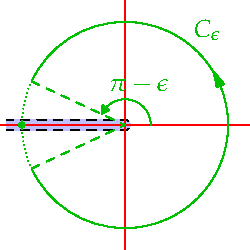
\includegraphics{contour-branch4}
		\end{minipage}
	
	  
	\end{enumerate}
\end{exercises}
\clearpage




\subsection[The Fundamental Theorem of Calculus]{Path-independence, the Fundamental Theorem \& Integral Estimation}\label{sec:ftc}

We start by revisiting an earlier example.

\begin{example*}{\ref{ex:basiccontour}, parts 2 \& 3}{}
	Let $F(z)=\frac 13z^3+z$ and observe that $F'(z)=z^2+1$. If $z:[a,b]\to \C$ parametrizes a smooth arc $C$ such that $z(a)=1$ and $z(b)=-1$, then Lemma \ref{lemm:chainsubs} shows that
	\begin{align*}
		\int_Cz^2+1\,\dz&=\int_a^b\bigl(z(t)^2+1\bigr)z'(t)\,\dt =\int_a^bF'\bigl(z(t)\bigr)z'(t)\,\dz =\int_a^b\diff tF\bigl(z(t)\bigr)\,\dt\\
		&=F\bigl(z(b)\bigr)-F\bigl(z(a)\bigr) = \frac 13z^3+z\Big|_1^{-1}\\
		&=-\frac 43-\frac 43=-\frac 83
	\end{align*}
	The contour integral is \emph{independent of the choice} of arc $C$, depending only on its \emph{endpoints.}
\end{example*}


\begin{defn}[lower separated=false, sidebyside, sidebyside align=top seam, sidebyside gap=0pt, righthand width=0.29\linewidth]{}{}
	Suppose $C$ is a contour in some path-connected $D\subseteq\C$ and that $f:D\to\C$. We say that $\int_Cf$ is \emph{path-independent} if its value depends only on the \emph{endpoints} of $C$ and not otherwise on the contour.\smallbreak
	Otherwise said, $\int_Cf=\int_{\widetilde C}f$ for any contour $\widetilde C$ with the same endpoints.
	\tcblower
	\flushright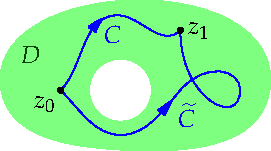
\includegraphics[scale=0.95]{ftc-5}
\end{defn}

	When $\int_C f$ is path-independent (and \emph{only} in such cases), it is permissible to write a contour integral with explicit limits: to write $\int_{z_0}^{z_1}f$ is to assert that the integral evaluates identically along any contour with endpoints $z_0,z_1$.\smallbreak

Before tackling the main result, we tidy up a connection between path independence and closed curves. You should have seen exactly this result in multi-variable calculus.

\begin{lemm}{}{pathindclosed}
	Let $f$ defined on a domain $D\subseteq\C$ be given. \textbf{Every} contour integral $\int_Cf(z)\,\dz$ over a contour in $D$ is path-independent if and only if $\int_Cf(z)\,\dz=0$ round \textbf{every} closed contour.
\end{lemm}

\begin{proof}
	\begin{description}\itemsep2pt
		\item[\normalfont ($\Rightarrow$)] Assume path-independence for all integrals $\int_Cf$ and let $C$ be a given \emph{closed} contour in $D$.\par
		\begin{minipage}[t]{0.8\linewidth}\vspace{-12pt}
			Choose any points $z_0,z_1\in C$ and decompose $C=C_1\cup C_2$ into two contours: from $z_0$ to $z_1$ and back again. Then,
			\begin{align*}
				\int_Cf(z)\,\dz&=\int_{C_1}f(z)\,\dz+\int_{C_2}f(z)\,\dz \tag{Theorem \ref{thm:basiccontour}, part 1}\\
				&=\int_{C_1}f(z)\,\dz-\int_{-C_2}f(z)\,\dz \tag{Theorem \ref{thm:basiccontour}, part 3}
			\end{align*}
			Since $C_1$ and $-C_2$ share the same endpoints, path-independence tells us that the integrals are equal, whence $\int_Cf=0$.
		\end{minipage} 
		\hfill
		\begin{minipage}[t]{0.19\linewidth}\vspace{-10pt}
			\flushright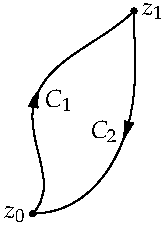
\includegraphics{ftc-1}
		\end{minipage}\par
		\item[\normalfont ($\Leftarrow$)] Conversely, suppose $\int_Cf(z)\,\dz=0$ round any closed contour in $D$, and let $C_1,-C_2$ be given contours in $D$ with the same endpoints $z_0,z_1$.\newline
		Plainly $C=C_1\cup C_2$ is a closed contour, and the previous calculation demonstrates path-independence:  $\int_{C_1}f(z)\,\dz=\int_{-C_2}f(z)\,\dz$.\qedhere
	\end{description}
\end{proof}


\goodbreak


In the above example, the existence of an \emph{anti-derivative} $F(z)=\frac 13z^2+z$ of $f(z)=z^2+1$ demonstrated path-independence, thus facilitating easy computation of the integral. This should seem familiar\ldots 

\begin{thm}{Fundamental Theorem}{ftc2}
	Let $f$ be continuous on an open domain. Then,
	\[
		\text{$f$ has an anti-derivative} \iff \text{all contour integrals $\textstyle\int_Cf$ are path-independent}
	\]
	In such situations, $\int_Cf(z)\,\dz=F(z_1)-F(z_0)$ where $F(z)$ is any anti-derivative of $f(z)$.
\end{thm}

The openness and continuity assumptions are necessary and will be used in the proof. In multi-variable calculus, the $(\Rightarrow)$ direction is often known as the Fundamental Theorem of Line Integrals.

\begin{examples}{}{}
	\exstart The function $f(z)=(z+i)^3$ has anti-derivative $F(z)=\frac 14(z+i)^4$. It follows that
	\[
		\int_0^{1-2i}(z+i)^4=\frac 14(z+i)^4\Big|_0^{1-2i}=\frac 14\left[(1-i)^4-i^4\right]=\frac 14(-4-1)=-\frac 54
	\]
	\emph{regardless} of the contour used to travel from $z=0$ to $1-2i$.

	\begin{enumerate}\setcounter{enumi}{1}
		\item Let $f(z)=z^{1/2}$ where we take the principal value. This has anti-derivative $F(z)=\frac 23z^{3/2}$.\par
		\begin{minipage}[t]{0.7\linewidth}\vspace{-10pt}
			If $C$ is any contour joining $z_0=1$ and $z_1=i$, which does not cross the branch cut, then
	  	\[
	  		\int_Cz^{1/2}\,\dz=\frac 23z^{3/2}\Big|_1^i=\frac 23(i^{3/2}-1^{3/2})=\frac 23\left(\polar{3\pi i}{4}-1\right)
	  	\]
	  	It is important to use the \emph{same (principal) branch} to evaluate the anti-derivative: since $z^{1/2}=e^{\frac 12\Log z}$, we also have $z^{3/2}=e^{\frac 32\Log z}$.
		\end{minipage}
		\hfill
		\begin{minipage}[t]{0.29\linewidth}\vspace{-10pt}
			\flushright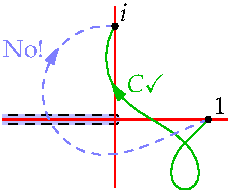
\includegraphics{contour-branch5}
		\end{minipage}
	  
	  \item Since $f(z)=\sin z$ has an anti-derivative $F(z)=-\cos z$ valid at all $z\in\C$, we see that $\int_C\sin z\,\dz=0$ round any closed curve $C$.
	  
	  \item (Example \ref{ex:int2pii}, cont)\lstsp Around the unit circle, $\oint_C\frac 1z\,\dz=2\pi i$ is non-zero. By the fundamental theorem, $f(z)=\frac 1z$ cannot have an anti-derivative on any domain containing said circle. But this is obvious from our discussion in Section \ref{sec:multivalued}: If an anti-derivative $F(z)$ existed, then
		\[
			\diff zF(z)=\frac 1z =\diff z\log z \implies F(z)=\log z+c \tag{Theorem \ref{thm:derivzeroconst}}
		\]
		for some branch of the logarithm, which contradicts the fact that no branch can be made single-valued on a path encircling the origin.\par
		\begin{minipage}[t]{0.7\linewidth}\vspace{-10pt}
			We can, however, use the fundamental theorem to evaluate $\int_C\frac 1z\,\dz$ over any contour staying within the domain of a single logarithm branch. In the picture, given the contour $C$, we choose the \textcolor{blue}{branch cut} shown and the logarithm with $-\frac{5\pi}3<\arg z<\frac\pi 3$:
			\begin{align*}
				\int_C\frac 1z\,\dz&=\log(1+i)-\log i =\log\sqrt 2\polar{\pi i}4-\log\polarn{3\pi i}2\\
				&=\ln\sqrt 2+\frac{\pi i}4-\frac{3\pi i}2=\frac 14(\ln 4+7\pi i)
			\end{align*}
		\end{minipage}
		\hfill
		\begin{minipage}[t]{0.29\linewidth}\vspace{-20pt}
			\flushright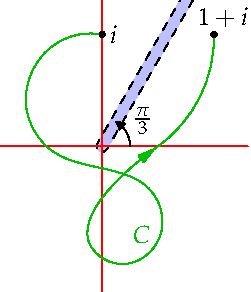
\includegraphics{contour-branch}
		\end{minipage}
	\end{enumerate}

\end{examples}


\goodbreak


\boldinline{Proving the Fundamental Theorem}

The forward direction is straightforward, though note the importance of a contour consisting of only \emph{finitely} many smooth arcs.


\begin{proof}
	\begin{description}
		\item[\normalfont ($\Rightarrow$)] Suppose $f$ has an anti-derivative $F$. Given a contour $C$ parametrized by a piecewise smooth function $z(t)$, write $C=C_1\cup\cdots\cup C_n$ where each $C_k$ is a smooth arc between endpoints $z_{k-1}=z(t_{k-1})$ and $z_k=z(t_k)$. By \textcolor{red}{Theorem \ref{thm:basiccontour}} and \textcolor{blue}{Lemma \ref{lemm:chainsubs}}, we see that
		\[
			\int_Cf \mathrel{\textcolor{red}{=}} \sum_{k=1}^n\int_{C_k}f
			=\int_{t_{k-1}}^{t_k}F'\bigl(z(t)\bigr)z'(t)\,\dt
			\mathrel{\textcolor{blue}{=}} \sum_{k=1}^n\bigl[F(z_k)-F(z_{k-1})\bigr] 
			=F(z_n)-F(z_0) \tag*{\phantom{\qedhere}}
		\]
	\end{description}
\end{proof}

The converse is similar to a standard proof of part I of the fundamental theorem from real analysis:
\[
	f\text{ continuous }\implies\diff x\int_a^xf(t)\,\dt=f(x)
\]
There are, however, a couple of extra subtleties: we must choose how to travel from one endpoint of an integral to the other (path-independence says it doesn't matter how); we also need to bound the modulus of a contour integral. This last isn't as trivial as it may seem\ldots
 
\begin{tcolorbox}[proofstyle]
	\begin{description}
		\begin{minipage}[t]{0.76\linewidth}\vspace{0pt}
			\item[\normalfont ($\Leftarrow$)] We prove when the domain $D$ is connected.\footnotemark{} Fix $z_0\in D$ and \emph{define} $F(z):=\int_{z_0}^zf(\zeta)\,\D\zeta$ where the integral is taken along \emph{any} curve (path-independence). We need to show that $\lim\limits_{w\to z}\frac{F(w)-F(z)}{w-z}=f(z)$ on $D$.\smallbreak
			Fix $z\in D$ and let $\epsilon>0$ be given. Since $f$ is continuous and $D$ open,
			\[
				\exists \delta>0\ \text{such that}\  \nm{\zeta-z}<\delta\implies \zeta\in D\ \text{and}\ \nm{f(\zeta)-f(z)}<\frac\epsilon 2
			\]
			Let $w\in D$ be such that $0<\nm{w-z}<\delta$. Evaluating along any curve joining $z,w$ (path-independence again), we obtain
			\[
				F(w)-F(z)=\int_z^wf(\zeta)\,\D\zeta
			\]
			\end{minipage}
			\hfill
			\begin{minipage}[t]{0.22\linewidth}\vspace{0pt}
				\flushright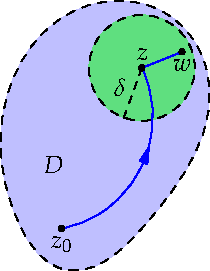
\includegraphics[scale=0.95]{ftc-2}
			\end{minipage}\medbreak
			For simplicity, we \emph{choose} the straight line segment from $z$ to $w$. The proof is almost complete:
			\begin{align*}
				\nm{\frac{F(w)-F(z)}{w-z}-f(z)}=&\nm{\frac 1{w-z}\int_z^wf(\zeta)-f(z)\,\D\zeta} = \frac 1{\nm{w-z}}\nm{\int_z^wf(\zeta)-f(z)\,\D\zeta}\\
				\textcolor{red}{\le}&\,\frac 1{\nm{w-z}}\nm{w-z}\frac\epsilon 2<\epsilon \tag*{\qedsymbol}
			\end{align*}
		\end{description}
\end{tcolorbox}

\footnotetext{If not, repeat the argument choosing a new $z_0$ for each connected component (`lump') of $D$.}

The second last \textcolor{red}{inequality} should give you pause. We are tempted to argue that
\[
	\nm{\int_z^wf(\zeta)-f(z)\,\D\zeta} \le \int_z^w\nm{f(\zeta)-f(z)}\D\zeta \le \int_z^w\frac\epsilon 2\,\D\zeta =\nm{w-z}\frac\epsilon 2
\]
This is fine in \emph{real} analysis (if $z\le w$), but is utter nonsense in \emph{complex}-land: the middle term
\[
	\int_z^w\nm{f(\zeta)-f(z)}\D\zeta=\int_a^b\nm{f\bigl(\zeta(t)\bigr)-f(z)}\zeta'(t)\,\dt
\]
\emph{need not be a real number}! We had better tidy this up\ldots

\goodbreak


\begin{thm}{Integral Estimation}{intbound}
	\exstart Suppose $w:[a,b]\to\C$ is piecewise continuous. Then
	\[
		\nm{\int_a^bw(t)\,\dt}\le\int_a^b\nm{w(t)}\dt
	\]
	\begin{enumerate}\setcounter{enumi}{1}
	  \item Suppose $C$ is a contour with length $L$, and let $f$ be piecewise continuous on $C$. Then $\nm{f(z)}$ is bounded by some $M\ge 0$ on $C$, and 
		\[
			\nm{\int_Cf(z)\,\dz}\le ML
		\]
	\end{enumerate}
\end{thm}

Part 2 justifies the suspect \textcolor{red}{inequality} in the proof of the Fundamental Theorem: $f(\zeta)-f(z)$ is bounded by $M=\frac\epsilon 2$ and the path of integration is the straight line of length $L=\nm{w-z}$.


\begin{proof}
	\begin{enumerate}
	  \item Let $\int_a^bw(t)\,\dt=re^{i\theta}$. Since $\theta$ is constant, $r=\int_a^be^{-i\theta}w(t)\,\dt$ is \emph{real.} In particular,
		\[
			r=\int_a^b\Re\bigl(e^{-i\theta}w(t)\bigr)+i\Im\bigl(e^{-i\theta}w(t)\bigr)\,\dt
			=\int_a^b\Re\bigl(e^{-i\theta}w(t)\bigr)\,\dt
		\]
		Appealing to $\Re z\le\nm z$, we see that
		\[
			\nm{\int_a^bw(t)\,\dt}
			=r =\int_a^b\Re(e^{-i\theta}w(t))\,\dt
			\le \int_a^b\nm{e^{-i\theta}w(t)}\,\dt
			=\int_a^b\nm{w(t)}\,\dt
		\]
		\item Parametrize the contour integral by $z:[a,b]\to\C$. Since $f(z(t))$ is piecewise continuous on a closed bounded interval, it is bounded and thus $M$ exists. But now,
		\begin{align*}
			\nm{\int_Cf(z)\,\dz}
			&=\nm{\int_a^bf\bigl(z(t)\bigr)z'(t)\,\dt}\le \int_a^b\nm{f\bigl(z(t)\bigr)z'(t)}\dt \tag{part 1}\\
			&\le \int_a^bM\nm{z'(t)}\dt
			=ML \tag*{\qedhere}
		\end{align*}
	\end{enumerate}
\end{proof}

While an explicit computation of arc-length is usually impractical, it is straightforward for circular or straight-line arcs. Indeed the estimation of integrals around circles is crucial for later sections.

\begin{examples}{}{estimates}
	\exstart On the straight line $C$ joining $z=4$ to $4i$, we see that\par
	\begin{enumerate}\setcounter{enumi}{1}
		\begin{minipage}[t]{0.65\linewidth}\vspace{-15pt}
		  \item[]
		  \[
		  	2\sqrt 2=\nm{2(1+i)}\le \nm z\le 4 \implies \nm{z+1}\le \nm z+1\le 5
		  \]
		  By the extended triangle inequality,
		  \[
		  	\nm{z^4+4}\ge \nm{\nm z^4-4}\ge \nm{(2\sqrt 2)^4-4}= 60
		  \]
		  Since $C$ has length $4\sqrt 2$, it follows that
		  \[
		  	\nm{\int_C\frac{z+1}{z^4+4}\,\dz} \le\frac{20\sqrt 2}{60}=\frac{\sqrt 2}{3}
		  \]
		\end{minipage}
		\hfill
		\begin{minipage}[t]{0.34\linewidth}\vspace{-15pt}
			\flushright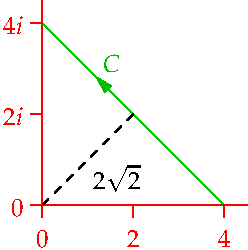
\includegraphics{bound-ex1}
		\end{minipage}
	
	  \item For the same function $f(z)=\frac{z+1}{z^4+4}$, consider the circle $C_R$ with radius $R>\sqrt[4]{4}$ centered at the origin. On $C_R$, we have $\nm{z}^4>4$; the triangle inequality tells us that
	  \[
	  	\nm{\frac{z+1}{z^4+4}}\le\frac{\nm{z}+1}{\nm{z^4}-4} =\frac{R+1}{R^4-4}\implies \nm{\oint_{C_R}\frac{z+1}{z^4+4}\,\dz}\le \frac{2\pi R(R+1)}{R^4-4}
	  \]
	  In particular, this approaches zero as $R\to\infty$.
	  
	  \begin{minipage}[t]{0.65\linewidth}\vspace{0pt}
			\item\label{ex:estimates3} Let $C_r$ be the circle with radius $r<2$ centered at $z=1$. Then
			\[
				\nm{z-1}=r\ \text{ and }\ \nm{z+1}=\nm{2-(1-z)}\ge 2-r
			\]
			from which
			\[
				\nm{\oint_{C_r}\frac 1{z^2-1}\,\dz}\le\frac{2\pi r}{(2-r)r}=\frac{2\pi}{2-r}\xrightarrow[r\to 0]{}\pi
			\]
		\end{minipage}
		\hfill
		\begin{minipage}[t]{0.34\linewidth}\vspace{0pt}
			\flushright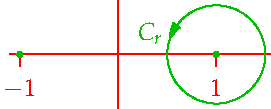
\includegraphics{bound-ex2}
		\end{minipage}\medbreak
		In Exercise \ref{exs:1-zsq}, it will be verified that $\oint_{C_r}\frac 1{z^2-1}\,\dz= i\pi$ for \emph{any} $r<2$.
	\end{enumerate}
	Examples 2 \& 3 are typical of the calculations dominating later sections.
\end{examples}


\begin{exercises}
	\exstart Evaluate each contour integral $\int_Cf(z)\,\dz$ using the fundamental theorem:

	\begin{enumerate}\setcounter{enumi}{1}
	  \item[]\begin{enumerate}
	    \item $f(z)=z^5$ where $C$ is the straight line from $z=1$ to $z=i$.
	    \item $f(z)=\dfrac 1z$ where $C$ is the pair of straight lines from $z=1$ to $-1-i$ to $-i$.
	    
	    \item $f(z)=iz\sin z^2$, where $C$ is the straight line from the origin to $z=i\sqrt\pi$.
	    
	    \item $f(z)=\dfrac 1{1+z^2}$ where $C$ is the straight line from $z=1$ to $2+i$.
	    \item $f(z)=\dfrac 1{\sqrt z}$ where $C$ is any path $z(t)$ with $\Re z>0$ joining $z=1+i$ and $z=4$.
	    
	    \item $f(z)=\operatorname{P.V.}z^{-1-2i}$ along the quarter circle $z(t)=e^{it}$ where $0\le t\le\frac\pi 2$.
		\end{enumerate}
		
		
	  \item Let $n\in\N_0$. Prove that for every contour $C$ from $z_0$ to $z_1$
	  \[
	  	\int_C z^n\,\dz=\frac 1{n+1}\left(z_1^{n+1}-z_0^{n+1}\right)
	  \]
	
	
	  \item If $C$ is a closed curve not containing $z_0$, and $n\in\Z\setminus\{0\}$, prove that $\int_C (z-z_0)^{n-1}\,\dz=0$.
	  
	
		\begin{minipage}[t]{0.75\linewidth}\vspace{0pt}
			\item Let $f(z)=z^{1/3}$ be the branch where $\arg z\in(-\frac\pi 2,\frac{3\pi}2)$. Evaluate the integral $\int_{C_1}f(z)\,\dz$ where $C_1$ is the curve shown in the picture.
			
			\item Evaluate $\int_{2i}^{1+i}\Log z\,\dz$ where the curve $C$ lies in the upper half-plane.\par
			(\emph{Hint: use integration by parts})
		\end{minipage}
		\hfill
		\begin{minipage}[t]{0.24\linewidth}\vspace{-10pt}
			\flushright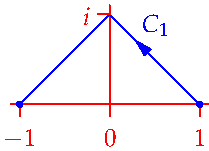
\includegraphics{ftc-3}
		\end{minipage}
		
		
			
		\item Evaluate $\int_{-1}^1z^{2-i}\,\dz$ where $z^{2-i}$ is the principal branch, and the integral is over any contour which, apart from its endpoints, lies above the real axis.
		
			  
	  \item Let $C$ be the arc of the circle $\nm z=2$ from $z=2$ to $2i$. Without evaluating the integral, show that
	  \begin{enumerate}
	  	\item $\displaystyle\nm{\int_C\frac{z+4}{z^3-1}\,\dz}\le \frac{6\pi}7$\qquad (b)\ \ $\displaystyle\nm{\int_C\frac{\dz}{z^2-1}}\le \frac{\pi}3$
	  \end{enumerate}
	  
	  
	  \item If $C$ is the straight line joining the origin to $1+i$, show that $\displaystyle\nm{\int_C z^3e^{2iz}\,\dz}\le 4$
	%   \[\nm{z^3e^{2iz}}=\nm{(1+i)^3t^3}\nm{e^{2i(1+i)t}}=\sqrt 8\nm t^3\nm{e^{2it}}\nm{e^{-2t}}\le\sqrt 8\]
	%   when $t\in[0,1]$. Since $C$ has length $\sqrt 2$, it follows that
	%   One could evaluate this explicitly using integration by parts, though it is time-consuming!
	
	
		\item If $C$ is the boundary of the triangle with vertices $0,3i$ and $-4$, prove that $\displaystyle\smash[b]{\nm{\oint_C(e^z-\cl z)\,\dz}}\le 60$\par
		(\emph{Hint: show that $\nm{e^z-\cl z}\le e^x+\sqrt{x^2+y^2}$\ldots})
		
		
		\item Let $C_R$ be the circle of radius $R>1$ centered at the origin. Prove that 
		\[
			\nm{\oint_{C_R}\frac{\Log z}{z^2}\,\dz} <2\pi\left(\frac{\pi +\ln R}R\right)
		\]
		and thus conclude that $\lim\limits_{R\to\infty}\oint_{C_R}\frac{\Log z}{z^2}\,\dz=0$.
		
		
	  \item\label{exs:1-zsq} (Hard)\lstsp We continue and expand Example \ref*{ex:estimates}.\ref{ex:estimates3}. Let $f(z)=\smash[b]{\frac 1{z^2-1}}$. 
	  \begin{enumerate}
	    \begin{minipage}[t]{0.7\linewidth}\vspace{-5pt}
	    	\item Explain why $F(z)=\frac 12\bigl(\Log(1-z)-\Log(1+z)\bigr)$ is an anti-derivative of $f(z)$ on the domain $D=\C\setminus\ell$ where $\ell$ consists of the two segments of the real axis where $\nm z\ge 1$.\smallbreak
	    Use $F(z)$ to evaluate $\int_0^{1+2i}f(z)\,\dz$ along \textcolor{blue}{any curve} in $D$.
	    \end{minipage}
	    \hfill
	    \begin{minipage}[t]{0.29\linewidth}\vspace{-25pt}
				\flushright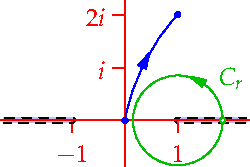
\includegraphics{ftc-6}
	    \end{minipage}
	    \par

		
			\begin{minipage}[t]{0.77\linewidth}\vspace{0pt}
	    	\item Show that $\oint_{C_r}f(z)\,\dz =i\pi$ where \textcolor{Green}{$C_r$ is a circle} of radius $r<2$ centered at $z=1$.\par
	   	 	(\emph{Hint: parametrize $z(t)=1+re^{it}$ where $-\pi<t<\pi$ and use $F(z)$})
	    
	    	\item Evaluate $\int_{C_2} f(z)\,\dz$ along a curve \textcolor{Purple}{$C_2$ passing to the \emph{right} of $z=1$} as in the picture. Compare your answer with parts (a) and (b).\par
	    	(\emph{Hint: you need a \textbf{different} branch of the log for one of the terms in $F(z)$})
			\end{minipage}
			\hfill
			\begin{minipage}[t]{0.22\linewidth}\vspace{0pt}
				\flushright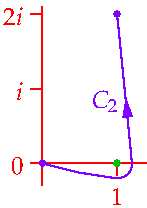
\includegraphics{ftc-4}
			\end{minipage}
	  \end{enumerate}
		
	\end{enumerate}
\end{exercises}

\clearpage



\subsection[Cauchy--Goursat \& the Integral Formula]{The Cauchy--Goursat Theorem and Cauchy's Integral Formula}

In this section we start to extend the fundamental theorem with the goal of more fully understanding and evaluating holomorphic functions. We first require another piece of topology.

\begin{defn}[lower separated=false, sidebyside, sidebyside align=top seam, sidebyside gap=0pt, righthand width=0.27\linewidth]{}{}
	A \emph{simply-connected} region $D$ is a path-connected set such that any simple closed curve $\textcolor{red}{C}\subseteq D$ may be shrunk to a point \emph{without leaving $D$}. Otherwise said, the  \textcolor{orange}{inside} of any such $\textcolor{red}{C}$ also lies in $D$.\smallbreak
	A non-simply connected region has \emph{holes}: e.g., the set $D$ pictured at the bottom of the page.
	\tcblower
	\flushright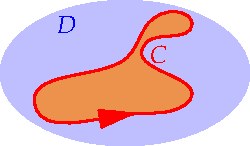
\includegraphics[scale=0.95]{simplyconnected}
\end{defn}

\begin{thm}{Cauchy--Goursat, version 1}{cauchygoursatv1}
	Suppose $C$ is a closed contour in a simply-connected region $D$. If $f$ is holomorphic on $D$, then $\int_Cf(z)\,\dz=0$.
\end{thm}

A basic proof invokes \emph{Green's Theorem} (from multi-variable calculus) after assuming that the real and imaginary parts of $f$ have continuous partial derivatives and that $C$ is simple. A proof without these assumption is significantly longer and more challenging.

\begin{lemm}{Green's Theorem}{}
	Suppose $D$ is a closed bounded simply-connected domain with boundary $C$ and that $P,Q:D\to\R$ have continuous partial derivatives. Then
	\[
		\oint_CP\,\dx+Q\,\dy=\iint_D\partials[Q]{x}-\partials[P]{y}\,\dA
	\] 
\end{lemm}

\begin{proof}[Sketch Proof of Cauchy--Goursat]
	Suppose $f(z)=u+iv$ has continuous partial derivatives and that $C$ is simple (assume WLOG that $C$ is positively oriented). Parametrize $C$ by $z(t)$, then
	\begin{align*}
		\oint_Cf(z)\,\dz&=\int_a^bf\left(z(t)\right)z'(t)\,\dt =\int_a^b\left(u(z(t))+iv(z(t))\right)\left(x'(t)+iy'(t)\right)\dt\\
		&=\int_a^bux'-vy'\,\dt+i\int_a^bvx'+uy'\,\dt\\
		&=\oint_Cu\,\dx-v\,\dy+i\oint_Cv\,\dx+u\,\dy \tag{definition of line integral in $\R^2$}\\
		&=\iint_D-v_x-u_y\,\dA+i\iint_Du_y-v_x\,\dA \tag{Green's Theorem}
	\end{align*}
	Both double integrals are zero by the Cauchy--Riemann equations. 
\end{proof}

\begin{minipage}[t]{0.64\linewidth}\vspace{0pt}
	To extend Cauchy--Goursat, we perform a sneaky trick. From the interior of a simple closed contour $\textcolor{blue}{C}$, remove the regions inside simple closed non-intersecting contours $\textcolor{red}{C_1,\ldots,C_k}$. Orient these clockwise so that the interior region $D$ lies to all contours' \emph{left.}\smallbreak
	By \textcolor{Green}{cutting} $D$ as indicated and traversing each cut twice in opposite directions, $\textcolor{blue}{C},\textcolor{red}{C_1,\ldots,C_k}$ and the \textcolor{Green}{cuts} may be joined to form a new simple closed contour. We may now apply Cauchy--Goursat\ldots
\end{minipage}
\hfill
\begin{minipage}[t]{0.35\linewidth}\vspace{0pt}
	\flushright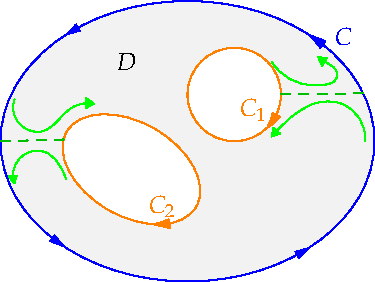
\includegraphics[scale=0.95]{multipleconnected1}
\end{minipage}

\goodbreak



\begin{cor}{Cauchy--Goursat, version 2}{}
	Suppose $C$ is a simple closed contour, oriented \textcolor{blue}{counter-clockwise}. Let $C_1,\ldots,C_k$ be non-intersecting simple closed contours in the interior of $C$, oriented \textcolor{orange}{clockwise}. If $f(z)$ is holomorphic on the region between and including $C$ and the interior boundaries $C_1,\ldots, C_k$, then
	\[
		\int_Cf(z)\,\dz+\sum_{j=1}^k\int_{C_j}f(z)\,\dz=0
	\]
\end{cor}

The power of this result lies in how it allows us to \emph{compare} integrals around different contours.

\begin{cor}{}{pathdef}
	Suppose $C_1,C_2$ are non-intersecting positively oriented simple closed contours. If $f$ is holomorphic on the region between and including the curves, then
	\[
		\oint_{C_1}f(z)\,\dz=\oint_{C_2}f(z)\,\dz
	\] 
\end{cor}

\begin{examples}{}{cauchygoursatexs}
	\exstart (Example \ref*{ex:estimates}.\ref{ex:estimates3}, cont.)\lstsp The function
	\begin{enumerate}\setcounter{enumi}{1}
	  \begin{minipage}[t]{0.75\linewidth}\vspace{-17pt}
			\item[]
			\[
				f(z)=\frac 1{z^2-1}
			\]
			is holomorphic \textcolor{blue}{on and between} any two circles $C_{r}$ centered at $z=1$ with radius $r<2$. Cauchy--Goursat thus confirms part of the conclusion of Exercise \ref*{sec:ftc}.\ref{exs:1-zsq}, that $\oint_{C_r}\frac 1{z^2-1}\,\dz$ is \emph{independent of the radius} $r$.\smallbreak
			We will shortly develop a better method to evaluate this integral.
		\end{minipage}
		\hfill
		\begin{minipage}[t]{0.24\linewidth}\vspace{-20pt}
		  \flushright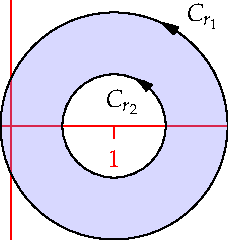
\includegraphics[scale=0.95]{cauchygoursat2}
		\end{minipage}

	  \item We compute the integral of $f(z)=\frac 1z$ around \emph{any} simple closed contour $C$ staying away from the origin.
	  \begin{itemize}
	    \item If the origin is \emph{outside} $C$, then $f$ is holomorphic on and inside $C$. By Cauchy--Goursat, we conclude that $\oint_C\frac 1z\,\dz=0$.
	    
	  	\begin{minipage}[t]{0.6\linewidth}\vspace{0pt}
	    	\item If the origin is \emph{inside}  $C$, then there is some minimum distance $d$ of $C$ to the origin. Choose any circle $C_r$ with radius $r<d$ centered at the origin. Since $f$ is holomorphic on the region $D$ between and including $C$ and $C_r$, we conclude that
				\[
					\oint_C\frac 1z\,\dz=\oint_{C_r}\frac 1z\,\dz =\int_0^{2\pi}\frac 1{re^{it}}ri e^{it}\,\dth=2\pi i
				\]
	  	\end{minipage}
	  	\hfill
	  	\begin{minipage}[t]{0.39\linewidth}\vspace{0pt}
	  		\flushright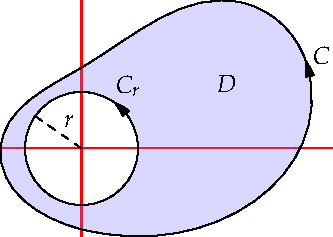
\includegraphics[scale=0.95]{cauchygoursat}
	  	\end{minipage}
  	\end{itemize}

  	More generally, if $C$ is a positively-oriented simple closed contour not containing $z_0$, then
  	\[
  		\oint_C\frac 1{z-z_0}\,\dz=
  		\begin{cases}
  			2\pi i&\text{if $z_0$ lies inside $C$}\\
  			0&\text{if $z_0$ lies outside $C$}
  		\end{cases}
  	\]
  	This example generalizes to perhaps the most powerful result in complex analysis\ldots
	\end{enumerate}
\end{examples}


\goodbreak



\begin{thm}{Cauchy's Integral Formula}{cauchyint}
	Suppose $f$ is holomorphic everywhere on and inside a simple closed contour $C$. If $z_0$ is any point inside $C$, then
	\[
		f(z_0)=\frac 1{2\pi i}\oint_C\frac{f(z)}{z-z_0}\,\dz
	\]
	More generally, $f$ is infinitely differentiable at $z_0$ with $n\th$ derivative
	\[
		f^{(n)}(z_0)=\frac{n!}{2\pi i}\oint_C\frac{f(z)}{(z-z_0)^{n+1}}\,\dz
	\]
\end{thm}

\begin{example}{}{}
	If $f(z)$ is a polynomial, we can check the integral formula explicitly by appealing to the Cauchy--Goursat Theorem and Exercise \ref*{sec:contour}.\ref{ex:intpowers}: if $C$ is a simple closed contour encircling $z_0$, then 
	\[
		\oint_C(z-z_0)^{n-1}\,\dz=
	 	\begin{cases}
	  	2\pi i&\text{if }n=0\\
	  	0&\text{otherwise}
	 	\end{cases}
	\]
	For instance, if $f(z)=3z^2+2$ and $z_0=0$, then
	\begin{gather*}
		%\frac 1{2\pi i}\oint_C\frac{3z^2+2}{z}\,\dz=\frac 1{2\pi i}\oint_C3z\,\dz+\frac 1{2\pi i}\oint_C\frac{2}{z}\,\dz =0+2=f(0)\\[5pt]
	%	\frac{1!}{2\pi i}\oint_C\frac{3z^2+2}{z^2}\,\dz=\frac 1{2\pi i}\oint_C3\,\dz+\frac 1{2\pi i}\oint_C\frac{2}{z^2}\,\dz =0+0=f'(0)\\[5pt]
		\frac{2!}{2\pi i}\oint_C\frac{3z^2+2}{z^3}\,\dz=\frac 2{2\pi i}\oint_C\frac 3z\,\dz+\frac 2{2\pi i}\oint_C\frac{2}{z^3}\,\dz =6+0=f''(0)
	\end{gather*}
\end{example}


\begin{proof}[Proof of the basic Integral formula\footnotemark]
	Let $\epsilon>0$ be given. Denote by $D$ the open region interior to $C$. Since $f$ is holomorphic it is also continuous. Combining these:\par
	\begin{minipage}[t]{0.75\linewidth}\vspace{-15pt}
		\[
			\exists\delta>0\ \text{such that}\ \nm{z-z_0}<\delta\implies z\in D\ \text{and}\ \nm{f(z)-f(z_0)}<\frac\epsilon 2
		\]
		Draw a circle $C_r$ of radius $r<\delta$ centered at $z_0$. This lies entirely in $D$. Since $\frac{f(z)}{z-z_0}$ is holomorphic between and on $C_r$ and $C$, Corollary \ref{cor:pathdef} tells us that
		\[
			\oint_C\frac{f(z)}{z-z_0}\,\dz=\oint_{C_r}\frac{f(z)}{z-z_0}\,\dz
		\]
		We need only bound an integral to complete the proof:
	\end{minipage}
	\hfill
	\begin{minipage}[t]{0.24\linewidth}\vspace{-10pt}
		\flushright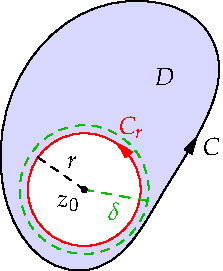
\includegraphics{cauchyintegral}
	\end{minipage}
	\begin{align*}
		\nm{\frac 1{2\pi i}\oint_{C}\frac{f(z)}{z-z_0}\,\dz-f(z_0)}
		&=\nm{\frac 1{2\pi i}\oint_{\textcolor{red}{C_r}}\frac{f(z)}{z-z_0}\,\dz-\frac{f(z_0)}{2\pi i}\oint_{\textcolor{red}{C_r}}\frac{1}{z-z_0}\,\dz}\\
		&=\nm{\frac 1{2\pi i}\oint_{\textcolor{red}{C_r}}\frac{f(z)-f(z_0)}{z-z_0}\,\dz}
		\underset{\ref{thm:intbound}}{\overset{\text{Thm}}{\le}} \frac 1{2\pi}\cdot\frac{\epsilon}{2r}\cdot 2\pi r
		<\epsilon %\tag*{\qedhere}
	\end{align*}
	since $\nm{z-z_0}=r$ and $\nm{f(z)-f(z_0)}<\frac\epsilon 2$ on $\textcolor{red}{C_r}$, which has circumference $2\pi r$.
\end{proof}

\footnotetext{%
	Informally, it appears as if the general formula follows by repeated differentiation (induction):
	\[
		f^{(n+1)}(z_0)=\diff{z_0}f^{(n)}(z_0) \overset{\text{???}}{=} \frac{n!}{2\pi i}\oint_C\partials{z_0}\frac{f(z)}{(z-z_0)^{n+1}}\dz = \frac{(n+1)!}{2\pi i}\oint_C\frac{f(z)}{(z-z_0)^{n+2}}\dz
	\]
	One cannot blindly bring a derivative inside an integral like this, so a formal proof is required; Exercise \ref{exs:cauchyintgeneral} offers a sketch.%
}
\goodbreak






\begin{examples}{}{intformula}
	We can use the integral formula to evaluate certain integrals that would be difficult if not impossible to evaluate by parametrization.
	\begin{enumerate}
	  \item The integral formula makes Example \ref*{ex:estimates}.\ref{ex:estimates3} and its extensions very easy: apply the formula to $f(z)=\frac{2\pi i}{z+1}$ around (say) the circle with radius 1 centered at $z=1$ to see that
  	\[
  		\oint_C \frac 1{z^2-1}\,\dz =\frac 1{2\pi i}\oint_C \frac{2\pi i}{(z+1)(z-1)}\,\dz =f(1) =i\pi 
  	\]
  	Indeed $\oint_C \frac 1{z^2-1}\,\dz =i\pi$ around any simple closed curve encircling $z=1$ but not $z=-1$.
	  
	  \item If $C$ is the circle centered at $z=i$ with radius 1, then $f(z)=\frac{3z\sin z}{z+i}$ is holomorphic on and inside $C$, whence
	  \begin{align*}
	  	\oint_C\frac{3z\sin z}{z^2+1}\,\dz 
	  	&=\oint_C\frac{3z\sin z}{(z+i)(z-i)}\,\dz
	  	=2\pi if(i)
	  	=2\pi i\frac{3i\sin i}{2i}
	  	=3\pi i\sin i\\
	  	&=\frac 32(e^{-1}-e^1)
	  \end{align*}
	  Contrast this with parametrizing $z(t)=i+e^{it}$ and attempting to evaluate directly!
 	  \[
 	  	\int_0^{2\pi}\frac{3(i+e^{it})\sin(i+e^{it})ie^{it}}{(i+e^{it})^2+1}\,\dt\ldots
	  \]
	  
	  \item Let $C$ be a simple closed contour staying away from $z_0=4$. Since $f(z)=\frac{3z^2+7}{e^z}$ is entire,
	  \[
	  	\oint_C\frac{3z^2+7}{e^z(z-4)}\,\dz=
	  	\begin{cases}
	  		0&\text{if $z_0=4$ is outside $C$}\\
	  		2\pi if(4)=110\pi ie^{-4}&\text{if $z_0=4$ is inside $C$}
	  	\end{cases}
	  \]
	  
	  \item Let $C$ be the circle of radius 2 centered at $z=1+i$. Then $g(z)=\frac 1{(z^2+1)^3}=\frac 1{(z+i)^3(z-i)^3}$ is holomorphic on and inside $C$, except at $z=i$. We conclude that
	  \[
	  	\oint_Cg(z)\,\dz=\oint_C\frac 1{(z+i)^3(z-i)^3}\,\dz=\frac{2\pi i}{2!}\diffat[^2]{z^2}{i}(z+i)^{-3} =12\pi i(2i)^{-5} =\frac{3\pi}{8}
	  \]
	\end{enumerate}
\end{examples}

We finish with a previously mentioned corollary of the integral formula.

\begin{cor}{Theorem \ref{thm:holoinfdiff}}{infdiff}
	Holomorphic functions are infinitely differentiable with all derivatives holomorphic. In particular, their real and imaginary parts have continuous partial derivatives of all orders.
\end{cor}


\begin{proof}
	If $f(z)$ is holomorphic at $w$, then it is holomorphic on an open set $D$ containing $w$. We may therefore choose a circle $C_r$ centered at $w$ lying inside $D$.\par
	The integral formula with $n=2$ says that the second derivative $f''(z_0)$ exists at every point $z_0$ inside $C_r$. Otherwise said, the derivative $f'(z)$ is holomorphic at $w$.\par
	Now induct to see the $f''(z)$ is holomorphic at $w$, etc.
\end{proof}

\goodbreak

Finally, note that if $f$ has an anti-derivative $F$, then $F$ is necessarily holomorphic and so, by the Corollary, is $f$ itself. Combining our results yields the following summary.

\begin{thm*}{Summary}
	Suppose $f$ is continuous on an open domain $D$ and that curves $C$ lie in $D$.
	\[
		\xymatrix @R20pt @C80pt{%
			\text{all}\ \oint_C f(z)\,\dz=0\quad \ar@{<=>}[d]_{\text{Lemma \ref*{lemm:pathindclosed}}}  & \quad f\ \text{holomorphic on $D$} \ar@{=>}[l]_{\text{Cauchy--Goursat}}^{\text{(if $D$ simply-connected)}}\\
			\text{all}\ \int_C f(z)\,\dz\ \text{path-independent} \quad \ar@{<=>}[r]_{\ \ \text{Fundamental Thm}} & \quad f\ \text{has an anti-derivative on $D$} \ar@{=>}[u]_{\text{Cauchy Integral Formula}} 
		}
	\]
\end{thm*}




 
% \begin{cor}{}{}
% Let $f$ be continuous on an open set $D$. If $\oint_C f(z)\,\dz=0$ for every closed contour in $D$, then $f$ is holomorphic.
% \end{cor}

% You might be fooled into thinking that this removes the need for the full version of the Cauchy--Goursat Theorem where we don't assume the continuity of the partial derivatives of $u,v$. You'd be wrong! The first step of the proof of the integral theorem requires Corollary \ref{cor:pathdef}. You could wriggle round this in another way however: first prove the Cauchy integral formula for \emph{circles} centered at each $z_0$ in an open domain, this shows that $f''(z)$ exists on $D$, which shows that $f'(z)$ and thus the partial derivatives of $u,v$ are continuous\ldots 


\begin{exercises*}
	\exstart Apply the Cauchy--Goursat Theorem to show that $\oint_Cf(z)\,\dz=0$ when the contour $C$ is the unit circle $\nm z=1$.
	\begin{enumerate}\setcounter{enumi}{1}
	  \item[]\begin{enumerate}
	    \item $\displaystyle f(z)=\frac{z^2}{z+3}$\qquad (b)\ \ $\displaystyle f(z)=ze^{-z}$\qquad (c)\ \ $\displaystyle f(z)=\Log(z+2)$
		\end{enumerate}
		
		
		\item Let $C_1$ be the square with sides the lines $x=\pm 1,y=\pm 1$, and $C_2$ the circle $\nm z=4$. Explain why
		\[
			\oint_{C_1}\frac 1{3z^2+1}\,\dz=\oint_{C_2}\frac 1{3z^2+1}\,\dz
		\]
		
		
		\item Let $C$ be the square with sides $x=0,1$ and $y=0,1$. Evaluate the integral $\oint_C\frac 1{z-a}\,\dz$ when:
		\begin{enumerate}
		  \item $a$ is \emph{exterior} to the square;
		  \item $a$ is \emph{interior} to the square.
		\end{enumerate}
		
		
		\item Let $C$ be the positively-oriented boundary of the half-disk $0\le r\le 1$, $0\le\theta\le\pi$ and define $f(z)=\sqrt z=\sqrt re^{i\theta/2}$ and $f(0)=0$ using the branch of $z^{1/2}$ with $-\frac{\pi}2<\theta<\frac{3\pi}2$. Prove that
		\[
			\oint_Cf(z)\,\dz=0
		\]
		by evaluating three contour integrals: over the semicircle, and over two segments of the real axis joining 0 to $\pm 1$. Why does Cauchy--Goursat not apply here?
		
		\item If $C$ is a positively-oriented simple closed contour, prove that the area enclosed by $C$ is
		\[\frac 1{2i}\oint_C\cl z\,\dz\]
		(\emph{Hint: Mirror the sketch proof of Cauchy--Goursat, even though $\cl z$ isn't holomorphic\ldots})
		
		
	  \item Let $C$ denote the boundary of the square with sides $x=\pm 2,y=\pm 2$. Evaluate the following:
	  \begin{enumerate}
	    \item $\displaystyle\oint_C\frac{e^{-\frac{\pi z}2}\,\dz}{z-i}$\qquad 
	   	(b)\ \ $\displaystyle\oint_C\frac{e^z+e^{-z}}{z(z^2+10)}\,\dz$\qquad 
	   	(c)\ \ $\displaystyle\oint_C\frac{z\,\dz}{3z+i}$\qquad 
	   	(d)\ \ $\displaystyle\oint_C\frac{\sec(z/2)}{(z-1-i)^2}\,\dz$
	  \end{enumerate}
	  
	  
	  \item Evaluate the integral $\oint_C g(z)\,\dz$ around the circle of radius 3 centered at $z=i$ when:
	  \begin{enumerate}
	    \item $\displaystyle g(z)=\frac 1{z^2+9}$\qquad (b)\ \ $\displaystyle g(z)=\frac 1{(z^2+9)^2}$
	  \end{enumerate} 
	  
	  
	  \item Prove that if $f$ is holomorphic on and inside a simple closed contour $C$ and $z_0$ is not on $C$, then
	  \[
	  	\oint_C\frac{f'(z)}{z-z_0}\,\dz =\oint_C\frac{f(z)}{(z-z_0)^2}\,\dz
	  \]
	  
	  
	  \item Properly justify the claim at the end of Example \ref{ex:intformula}.1, that
	  \[
	  	\oint_{C}\frac{1}{z^2-1}\dz=i\pi
	  \]
	  when $C$ is \emph{any} simple closed curve encircling $z=1$ but not $z=-1$. What happens if instead $C$ encircles $z=-1$ but not $z=1$?
	  
	  
	  \item Suppose we have a polynomial $p(z)=\sum\limits_{k=0}^na_k(z-z_0)^k$ centered at $z_0$.
	  Use Cauchy's integral formula to prove that $a_k=\frac{p^{(k)}(z_0)}{k!}$ is the usual Taylor coefficient.
	  
	  
	  \item Let $C$ be the unit circle $z=e^{i\theta}$ where $-\pi<\theta\le\pi$ and suppose $a\in\R$ is constant. By first evaluating $\oint_Cz^{-1}e^{az}\,\dz$, prove that
	  \[
	  	\int_0^\pi e^{a\cos\theta}\cos(a\sin\theta)\,\dth=\pi
	  \] 
		
		  
	  \item\begin{enumerate}
	     \item Suppose that $f(z)$ is \emph{continuous} on and inside a simple closed contour $C$. Prove that the function $g(z)$ defined by
	    \[
	    	g(z_0):=\frac 1{2\pi i}\oint_C\frac{f(z)}{z-z_0}\,\dz
	    \]
	    is holomorphic at every point $z_0$ inside $C$ and that
	    \[
	    	g'(z_0):=\frac 1{2\pi i}\oint_C\frac{f(z)}{(z-z_0)^2}\,\dz
	    \]
	    (\emph{Hint: consider the formula in part (b) of the next question, after replacing the first two $f$'s by $g$})
	    
	    \item If $f(z)=x(1-x)(1-y)$ and $C$ is the square with vertices $0,1,1+i,i$ compute $g(z_0)$.
	  \end{enumerate}
	
	  
		\item\label{exs:cauchyintgeneral} We prove the 1\st\ derivative version of Cauchy's integral formula. As previously, let $\delta>0$ be such that $\nm{w-z_0}<\delta\implies w\in D$.
		\begin{enumerate}
		  \item If $\nm{\Delta z}<\delta$ and $z\in C$ explain why
		  \begin{enumerate}
		    \item $\nm{z-z_0}\ge \delta$
		    \item $\nm{z-z_0-\Delta z}>0$ 
		  \end{enumerate}
		  \item Use the basic integral formula on $C$ to evaluate $f(z_0+\Delta z)-f(z_0)$ and thus prove that
		  \[
		  	\nm{\frac{f(z_0+\Delta z)-f(z_0)}{\Delta z}-\frac 1{2\pi i}\oint_C\frac{f(z)}{(z-z_0)^2}\,\dz} \le \frac{ML}{2\pi(\delta-\Delta z)\delta^2}\nm{\Delta z}
		  \]
		  where $M$ is an upper bound for $\nm{f(z)}$ on $C$, and $L$ is the length of $C$. Hence conclude that $f'(z_0)=\frac 1{2\pi i}\oint_C\frac{f(z)}{(z-z_0)^2}\,\dz$.
		\end{enumerate}
		If you want a challenge, try to do the same thing for higher derivatives!
		
	\end{enumerate}
\end{exercises*}
  
    
\clearpage\iffalse


\subsection{Liouville's Theorem and The Maximum Modulus Principle}

In this section we deduce several powerful corollaries of Cauchy's integral formula. The first is a straightforward combination of the integral formula with integral estimation (Theorem \ref{thm:intbound}).

\begin{lemm}{Cauchy's Inequality}{}
	If $f$ is holomorphic on and inside the circle $C$ of radius $R$ centered at $z_0$, and $\nm{f(z)}\le M$ on $C$, then
	\[
		\nm{f^{(n)}(z_0)}
		=\frac{n!}{2\pi}\nm{\oint_{C}\frac{f(z)}{(z-z_0)^{n+1}}\,\dz}
		\le \frac{n!M}{R^n}
	\]
\end{lemm}

This seems innocuous, but it has surprising applications. If $f$ is entire and bounded ($\nm{f(z)}\le M$ for all $z$), then Cauchy's inequality applies for \emph{any} circle centered at \emph{any} $z_0$:
\[
	\forall z_0\in\C,R>0,\ \nm{f'(z_0)}\le\frac MR 
	\implies \forall z_0,\ f'(z_0)=0 
	\overset{\text{Thm}}{\underset{\text{\ref{thm:derivzeroconst}}}{\implies}}
	f(z)\text{ constant}
\]

\begin{thm}{Liouville}{}
	Every bounded, entire function is constant.
\end{thm}

Liouville's Theorem is the key ingredient in perhaps the simplest proof of a very famous result.

\begin{cor}{Fund.{} Thm.{} of Algebra}{}
	Every non-constant polynomial has a root in $\C$. %Moreover, every such $p(z)$ factors uniquely up to ordering as a product of linear factors:
	%\[p(z)=a(z-z_1)\cdots(z-z_n)\] 
\end{cor}

\begin{proof}
	WLOG suppose a non-constant polynomial $p(z)=z^n+\sum_{k=0}^{n-1}a_kz^k$ is monic. We assume, for contradiction, that $p(z)=0$ has no solutions. It follows that is $\frac 1{p(z)}$ is \emph{entire}. Our strategy is to establish that $\frac 1{p(z)}$ is also \emph{bounded}; since $p(z)$ is non-constant, this contradicts Liouville's Theorem.\par
	In fact it is enough to bound $\frac 1{p(z)}$ for all \emph{large} $z$: that is, we want to find some $R>0$ such that
	\[
		\nm z>R\implies \frac 1{p(z)}\text{ bounded}
	\]
	This is since $\frac 1{p(z)}$, being continuous, is automatically bounded on any disk $\nm z\le R$ (compactness, Theorem \ref{thm:compactconnected}). So how do we find a suitable $R$? Everything follows from the triangle inequality,
	\[
		\nm z>R \implies
		\nm{p(z)}=\nm z^n\nm{1+\sum_{k=0}^{n-1}\frac{a_k}{z^{n-k}}} 
		\ge \nm z^n\nm{1-\nm{\sum_{k=0}^{n-1}\frac{a_k}{z^{n-k}}}}
	\]
	To complete the proof, we need only choose $R$ such that $\nm{\sum_{k=0}^{n-1}\frac{a_k}{z^{n-k}}}\le \sum_{k=0}^{n-1}\textcolor{red}{\frac{\nm{a_k}}{\nm z^{n-k}}}\le\frac 12$, for then
	\[
		\nm z>R\implies \nm{p(z)}\ge \frac 12R^n\implies \frac 1{\nm{p(z)}}\le \frac 2{R^n}
	\]
	is bounded. It is sufficient to force each term in the \textcolor{red}{above sum} to be $\le \frac 1{2n}$, as may be accomplished (see Exercise \ref{exs:fundthmalg}) by defining
	\[
		R:=\max_{}\left\{(2n\nm{a_k})^{\frac 1{n-k}}:0\le k<n\right\} \tag*{\qedhere}
	\]
\end{proof}



The proof used the fact that a continuous function $f$ on a compact (closed, bounded) domain $K$ is bounded (Theorem \ref{thm:compactconnected}). As you should recall from real analysis, the least upper bound is achieved:
\[
	\exists z_0\in K\text{ such that } \nm{f(z_0)}=\sup\bigl\{\nm{f(z)}:z\in K\bigr\}
\] 
For \emph{holomorphic} functions, something more restrictive and surprising is true: the maximum modulus of a holomorphic function on a compact domain is always and only achieved at an \emph{edge point}.

\begin{example}{}{}
	Let $f(z)=e^z$ on the unit disk $\nm z\le 1$. Then $\nm{f(z)}=e^x$, whence the maximum modulus $\nm{f(1)}=e$ occurs at $z=1$, on the edge of the disk.
\end{example}

The theorem establishing this important observation is usually stated a little differently.

\begin{thm}{Maximum Modulus Principle}{}
	Suppose $f$ is holomorphic and non-constant on a \emph{connected, open} domain $D$. Then $\nm{f(z)}$ has no maximum value on $D$.
\end{thm}


\begin{proof}
	We start by demonstrating the contrapositive of a special case.\par
	\begin{minipage}[t]{0.79\linewidth}\vspace{-6pt}
		Fix $\delta>0$, assume $f$ is holomorphic on and inside $\cl{B_0}:=\{z:\nm{z-z_0}\le\delta\}$ and that \textcolor{red}{$\nm{f(z)}$ attains its maximum at $z_0$}. We prove that $f(z)$ is \emph{constant} on $\cl{B_0}$.\smallbreak
		Let $r\le\delta$ and apply the integral formula to the circle \textcolor{Brown}{$C_{r}$} \ ($z(t)=z_0+re^{it}$):
	\end{minipage}
	\hfill
	\begin{minipage}[t]{0.2\linewidth}\vspace{-21pt}
		\flushright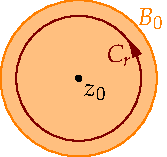
\includegraphics[scale=0.95]{maxmod2}
	\end{minipage}\par
	\vspace{-10pt}
	\begin{align*}
		\nm{f(z_0)}
		&=\frac 1{2\pi}\nm{\oint_{C_{r}}\frac{f(z)}{z-z_0}\,\dz}
		=\frac 1{2\pi}\nm{\int_0^{2\pi}\frac{f(z_0+r e^{it})}{r e^{it}}ir e^{it}\,\dt}
		=\frac 1{2\pi}\nm{\int_0^{2\pi}f(z_0+r e^{it})\,\dt}\\
		&\le \frac 1{2\pi}\int_0^{2\pi}\nm{f(z_0+r e^{it})}\dt \tag{Theorem \ref{thm:intbound}}\\
		&\mathrel{\textcolor{red}{\le}} \frac 1{2\pi}\int_0^{2\pi}\nm{f(z_0)}\,\dt =\nm{f(z_0)} \tag{$\nm{f(z_0)}$ is the \textcolor{red}{maximum} of $\nm{f(z)}$}
	\end{align*}
	Both inequalities are therefore \emph{equalities,} the \textcolor{red}{second} of which now becomes
	\[
		\int_0^{2\pi}\nm{f(z_0)}-\nm{f(z_0+r e^{it})}\dt=0
	\]
	Since the integrand is \textcolor{red}{non-negative} and continuous, it must be zero. But then $\nm{f(z)}=\nm{f(z_0)}$ on \emph{all such circles} $C_r$, whence $\nm{f(z)}$ is \emph{constant} on $\cl{B_0}$. By Corollary \ref{cor:modimpliesconst}, $f(z)$ is also constant on $B_0$.\medbreak
	
	Now suppose $f$ is holomorphic on some connected open set $D$ and that $\nm{f(z)}$ attains its maximum at $z_0$. Let $w\in D$ be any other point and join $z_0$ to $w$ by a smooth arc \textcolor{Green}{$C$}.\par
	\begin{minipage}[t]{0.62\linewidth}\vspace{-2pt}
		Following Exercise \ref*{sec:opensets}.\ref{exs:finitesubcover}, we may cover $C$ with \emph{finitely many} closed disks $\cl{B_0},\cl{B_1},\ldots,\cl{B_n}\subset D$ of some radius $\delta$, indexed so that each center $z_k$ lies in one of the previous disks: indeed we need at most $\frac{\text{length}(C)}{\delta}$ disks for this.\smallbreak
		By the special case, $f(z)$ is constant on $\cl{B_0}$. Since $z_1\in C\cap\cl{B_0}$, we see that $\nm{f(z_1)}=\nm{f(z_0)}$ is also the maximum modulus on $D$. The special case now says that $f(z)$ is constant on $\cl{B_0}\cup \cl{B_1}$.
	\end{minipage}
	\hfill
	\begin{minipage}[t]{0.36\linewidth}\vspace{-5pt}
		\flushright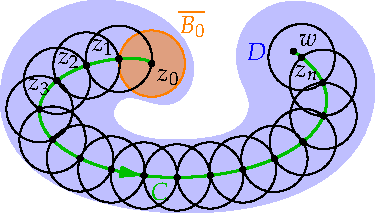
\includegraphics[scale=0.95]{maxmod}
	\end{minipage}\medbreak
	Continuing in this fashion (essentially induction), we conclude that $f(z)=f(z_0)$ is constant on $\cl{B_0}\cup\cdots\cup\cl{B_n}$. In particular $f(w)=f(z_0)$. Since $w$ was arbitrary, $f(z)$ is constant on $D$.
\end{proof}


\begin{example}{}{modulusexplicit}
	Let $f(z)=2z^2+i$ on the upper semi-disk with radius 1. There are two boundaries:\par
		\begin{minipage}[t]{0.65\linewidth}\vspace{0pt}
			\begin{itemize}
			  \item $y=0$: plainly $\nm{f(z)}=\sqrt{4x^4+1}$ is maximal at $z=\pm 1$.
				\item $r=1$: write $f(z)=2e^{2i\theta}+i$ from which
			  \[
			  	\nm{f(z)}=\sqrt{(2\cos 2\theta)^2+(2\sin 2\theta+1)^2} =\sqrt{5+4\sin 2\theta}
			  \]
			  which is maximal when $\theta=\frac\pi 4$ with $\nm{f(\polar{i\pi}4)} =3$.
			\end{itemize}
		\end{minipage}
		\hfill
		\begin{minipage}[t]{0.32\linewidth}\vspace{-10pt}
			\flushright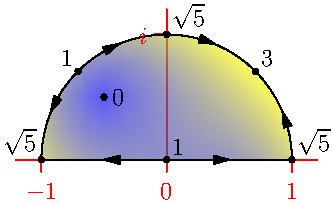
\includegraphics[scale=0.95]{maxmod3}
		\end{minipage}\smallbreak
		The color indicates the value of $\nm{f(z)}$, and the arrows its direction of increase on the boundary. 
\end{example}

 
\begin{exercises}
	\hangindent\doubleind
	\textup{1.} \ (a) \ Suppose $f$ is entire and that $\nm{f(z)}\le c\nm z$ for some constant $c\in\R^+$. Prove that $f(z)=kz$ where $k\in\C$ satisfies $\nm k\le c$.
	
	\begin{enumerate}\setcounter{enumi}{1} 
	  \item[]\begin{enumerate}\setcounter{enumii}{1} 
	    \item What can you say about $f$ if it is entire and there exists some linear polynomial $cz+d$ with $c\neq 0$ such that $\nm{f(z)}\le\nm{cz+d}$ for all $z\in\C$?
	  \end{enumerate}
	  
	  
	  \item If $f(z)=u+iv$ is entire and $u(x,y)$ is bounded above, apply Liouville's Theorem to $\exp(f(z))$ to prove that $u$ is constant.
	  
	  
	  \item Let $f(z)$ be a non-zero holomorphic function on a closed bounded domain. By considering $g(z)=\frac 1{f(z)}$, show that the minimum value of $\nm{f(z)}$ also occurs on the boundary.
	  
	  
	  \item Find the maximum and minimum values of $\nm{z^2+4i}$ on the unit disk $\nm z\le 1$.
	  
	  
	  \item On the rectangle $0\le x\le\pi$, $0\le y\le 1$, show that $\nm{\sin z}$ is maximal at the point $z=\frac\pi 2+i$.\par
	  (\emph{Hint: first show that $\nm{\sin z}^2=\sin^2\!x+\sinh^2\!y$})
	  
	  
	  \item Revisit the standard method from multivariable calculus (compute $\nabla\nm{f(z)}^2$) to check that the maximum value of $\nm{2z^2+i}$ in Example \ref{ex:modulusexplicit} really does occur on the boundary.
	
	
	  \item\label{exs:fundthmalg} Complete the proof of the fundamental theorem of algebra: 
	  \begin{enumerate}
	    \item Verify that $R:=\max\bigl\{(2n\nm{a_k})^{\frac 1{n-k}}:0\le k<n\bigr\}$ is \emph{positive.}
	    \item Prove that $\nm z>R\implies \forall k,\ \frac{\nm{a_k}}{\nm z^{n-k}}<\frac 1{2n}$.
	  \end{enumerate}
	    
	    
	  \item\begin{enumerate}
	    \item Prove the factor theorem: if $p(z_1)=0$, then $p(z)=(z-z_1)q(z)$ for some polynomial $q(z)$.\par
	    (\emph{Hint: This follows easily from the division algorithm: if $\deg p\ge \deg g$, then there exist unique polynomials $q(z),r(z)$ for which
	    \[
	    	p(z)=g(z)q(z)+r(z)\quad\text{and}\quad \deg r<\deg g
	    \]
	    For a challenge, prove some version of this sufficient for our needs\ldots)
	    }
	    \item Prove that a degree $n\ge 1$ polynomial $p(z)$ factors uniquely over $\C$: up to order, there exist unique $a,z_1,\ldots,z_n\in\C$ such that
	    \[
	    	p(z)=a(z-z_1)\cdots(z-z_n)
	    \]
	  \end{enumerate}
	\end{enumerate}
\end{exercises}

\fi